\input preamble.tex
\begin{centering}
\Huge{\textbf{Prøve 02 i Styringsteknikk}}\\
\end{centering}
\vskip 2cm 
\begin{itemize}
	%\item utføre arbeid på automatiserte anlegg fagmessig, nøyaktig og i overensstemmelse med krav til helse, miljø og sikkerhet og rutiner for kvalitetssikring og internkontroll
	%\item utføre risikovurdering og vurdere tiltak for ivaretakelse av person– og maskinsikkerhet
	%\item vurdere hvilke regelverk og normer som gjelder for arbeidet som skal utføres og anvende dette
	%\item planlegge, utføre, vurdere kvalitet, sluttkontrollere og dokumentere arbeidet
	\item planlegge, programmere, montere og idriftsette programmerbare styresystemer
	\item endre og tilpasse skjermbilder for grensesnitt mellom menneske og maskin
	%\item anvende ulike elektroniske kommunikasjonssystemer i automatiserte anlegg
	%\item vurdere datasikkerhet i automatiserte anlegg
	%\item tegne, lese og forklare instrumenterte prosessflytskjemaer og bruke annen relevant dokumentasjon for automatiserte anlegg
	%\item montere, konfigurere, kalibrere og idriftsettelse digitale og analoge målesystemer
	%\item idriftsette og optimalisere regulatorer basert på prosessbehov
	%\item montere og idriftsette ulike typer pådragsorganer med tilhørende forstillingselementer og hjelpeutstyr
	%\item programmere, idriftsette samt gjøre rede for roboters funksjon og anvendelse i produksjonsanlegg
	%\item måle fysiske størrelser i automatiserte anlegg
	%\item feilsøke og rette feil i automatiserte anlegg
	%\item bruke gjeldende regelverk og normer for elektriske installasjoner på maskiner
	%\item bruke gjeldende regelverk og normer for installasjon av elektroniske kommunikasjonssystemer
	%\item beskrive ulike vedlikeholdssystemer og -rutiner knyttet til automatiserte anlegg, og anvende et av disse
	%\item redegjøre for bedriftens organisasjonsoppbygging og bedriftens verdiskapning i et samfunnsperspektiv
	%\item dokumentere egen opplæring i automatiseringssystemer
\end{itemize}
\vskip 2.5pt 
Hjelpemidler:\begin{itemize}[noitemsep]
	\item Oppgave 1-4: Kalkulator og formelark
	\item Oppgave 5-9 Alle ikke kommuniserende
\end{itemize}

\vskip 5pt 
\vskip 10pt 
Alle ark som leveres inn skal ha elevens navn.
\vskip 2.5pt 
Oppgave 1-4 skal leveres på papir, etter levering kan eleven ta frem PC og svare på oppgave 9. 
\vskip 2.5pt 
Oppgave 5-9 skal utføres i samme codesys project. (slik at det bare leveres inn en fil.)
Når oppgave 5-9 skal leveres kan elevene slå på trådløst nettverkt og sende oppgaven på mail til:
\vskip 2.5pt 
fred-olav.mosdal@skole.rogfk.no
\vskip 2.5pt 
I emnefeltet skal det stå: PLS Prøve
\vskip 2.5pt
Oppgaven SKAL sendes fra skolemailen. 
\vskip 2cm   
Konaktinformasjon:
\begin{itemize}[noitemsep]
	\item Kontaktlærer: Fred-Olav Mosdal
	\item TLF: 90507684
\end{itemize}


\vfil \eject
%Slutt forside
Oppgave 1 (6p)%Navngi
\vskip 2.5pt 
a) Nevn 3 action qualifiers og beskriv hva de gjør.
\vskip 2.5pt 

\begin{tikzpicture}
	\draw[step=0.5cm,gray!20,thin]  grid (17,10) ;
\end{tikzpicture}
\vskip 2.5pt 
b) Hvilke to typer steg har vi i SFC.
\vskip 2.5pt 

\begin{tikzpicture}
	\draw[step=0.5cm,gray!20,thin]  grid (17,10) ;
\end{tikzpicture}
\vfil\eject

Oppgave 2 (6p) %Definisjoner
\vskip 2.5pt 
a) Hva en en transission i sekvensielle funknsjonskart?\\
\vskip 2.5pt 

\begin{tikzpicture}
	\draw[step=0.5cm,gray!20,thin]  grid (17,11) ;
\end{tikzpicture}
\vskip 10pt 
b) Hva er en action i sekvensielle funksjonskart?\\
\vskip 2.5pt 

\begin{tikzpicture}
	\draw[step=0.5cm,gray!20,thin]  grid (17,11) ;
\end{tikzpicture}
\vskip 2.5pt 
\vskip 2.5pt 
\vfil\eject

Oppgave 3 (6p)%Enkel utregninger.
\vskip 2.5pt 
En Allen-Bradley SLC500 PLS blir bukt som regulator for en ovn. Prosessvariabelen TT01 er tilkoblet channel 0 på en firekanals inngangmodul. Transmitteren har et måleområde på 100-600°C. Vi må skallere denne verdien slik at den kan brukes til å gengi temperaturen på på HMI. HMI symbolet som skal brukes skal tilføres en verdi på 1000-6000. Komma tilføres automatisk av symbolet.  


$$\includegraphics[width=15.5cm]{i03648x01.eps}$$

Prosessbildet forteller at inngangmodulen gir en int verdi på 4000 ved 4mA og 20000 ved 20mA. 

\vskip 10pt
\vfil\eject
a) Lag en matematisk formel for konverteringen av temperaturen. 
\vskip 10pt

\begin{tikzpicture}
	\draw[step=0.5cm,gray!20,thin]  grid (17,11) ;
\end{tikzpicture}
\vskip 10pt 
b) tegn et ladder program som viser hvordan denne formelen kan implementeres. 

\vskip 10pt 

\begin{tikzpicture}
	\draw[step=0.5cm,gray!20,thin]  grid (17,11) ;
\end{tikzpicture}
\vfil\eject
Oppgave 4 (6p) %Tegneoppgaver(blokkskjema skisse osv. 
\vskip 2.5pt 
a) Tegn en sekvens med parallelle veier\\
\vskip 10cm
b) Tegn en sekvens med to valgbare veier\\
\vskip 5cm 
% Her kommer oppgaver som skal kreve forklaringer eller forståelse
\vfil\eject

Oppgave 5 til 8 bygger på hverandre.
\vskip 2.5pt
 Tegningen nedenfor viser anlegget det er snakk om. Det skal lages en HMI som gjør det mulig å teste programmet. Det vil si at alle brytere, lamper og informasjon må vises på HMI. 
 \vskip 5pt 
$$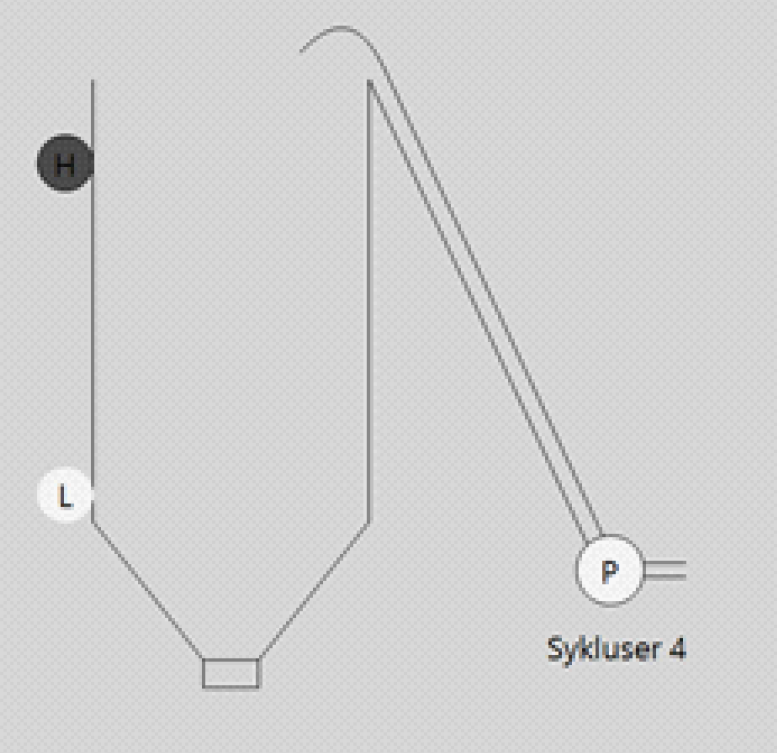
\includegraphics[width=0.5\textwidth]{i08012x01.png}$$

\vskip 5pt 
En kornsilo skal fyllest ved hjelp av en pumpe. Der er to nivåvakter i hver silo (L og H) disse gir \verb|TRUE| når nivået ligger over giveren.

\vskip 5pt 
Virkemåte: Pumpa i en silo skal alltid starte når nivået er under
minimum og stoppe når nivået går over maksimum for siloen.

\vskip 1cm
Oppgave 5 (6p) %Kombinatorisk programmering
\vskip 2.5pt 

Anlegget settes i drift med en Start knapp og stoppes med en Stoppknapp.
Når anlegget er satt i drift og nivået er under L startes pumpe P.
Denne går til nivået når H. Slik fortsetter det til driften av anlegget
stoppes med stoppknappen.
\vskip 5pt 
Oppgave 6 (6p) % Tegn og forklar virkemåte
\vskip 2.5pt 
Legg til Auto/Manuell styring av pumpe

\vskip 10pt 
Oppgave 7 (6p) % Tegn og forkalr virkemåte. 
\vskip 2.5pt 
Lag en Visualisering som ligner den på bildet, alle funksjoner som beskrives i oppgaven kommer i tillegg. 

\vskip 10pt 
Oppgave 8 (6p) % Regneoppgave
\vskip 2.5pt 
Legg til en teller for totalt antall sykluser på pumpe (skal vises på skjerm). 
\vskip 1cm

\vskip 5pt 
\vskip 0.5cm
\begin{tabular}{|c|c|c|c|}
\hline 
Tilkoblet utstyr & IO på RIO & Variabel & Beskrivelse av tilkoblet utstyr\tabularnewline
\hline 
\hline 
Start Knapp & Bryter1 & Start & \tabularnewline
\hline 
Stopp Knapp & Bryter2 & Stopp & \tabularnewline
\hline 
H Sensor & Bryter3 & LevelHigh & \tabularnewline
\hline 
L Sensor & Bryter4 & LevelLow & \tabularnewline
\hline 
Drifts Lys & Lys1 & Drift & \tabularnewline
\hline 
Pumpe Lys & Lys2 & Pumpe & \tabularnewline
\hline 
Alarm Lys & Lys3 & AlarmLys & \tabularnewline
\hline 
Alarm Lyd & Lys4 & AlarmLyd & \tabularnewline
\hline 
\end{tabular}

\vfil\eject
Oppgave 9 (12p) \\ %skal beskrive hvordan en jobb skal utføres. (Planlegg, besriv hvordan du ville gjenomført og dokumenter jobben)

Hydraulisk Pressemater 

\vskip 5pt 
Ei hydraulisk presse stanser deler ut av ei plate som føres inn av
en hydraulisk mate-mekanisme. Plata kommer fra et kveilanlegg som
ligger forut (til venstre) for dette matesystemet.

\vskip 5pt 
Skissa under viser de fire sylindrene som arbeider sammen under den kontinuerlige operasjonen. Før den automatiske funksjonen kan starte må plata være matet fram manuelt slik at den går gjennom pressa mens denne er åpen. Begge klemsylindrene (S1 og S3) har klemt til og vi har signal på både I 01 og I 04 og matesylinderen er i sin minus stilling (I 03). 
\vskip 5pt 

Funksjonen I automatikk er følgende: Pressa går ned og stanser ut delen som faller ned I samleboksen under verktøyet. Samtidig mens pressa går løsner S1 taket, matesylinderen S2 går til sin +posisjon (I 02) og så klemmer S1 til igjen. Når pressa er kommet opp igjen slipper S3 taket og matesylinderen går fram til sin \textendash posisjon (I 03). Når det skjer klemmer S3 til igjen og pressa går på nytt. 
\vskip 5pt 

Lag denne funksjonen i SFC
\vskip 5pt 
$$\includegraphics[width=15.5cm]{/Sekvensoppgave05.eps}$$
$$\includegraphics[width=15.5cm]{/Sekvensoppgave06.eps}$$;



\vskip 5pt 
\includepdf[page=-,angle=90]{../eq/afgvformler.pdf}
\end {document}
